\documentclass[border=8pt,tikz]{standalone}
\usepackage{tikz}
% Shared TikZ style for Chapter 5 diagrams.
% Inputted by every standalone diagram file.

\usetikzlibrary{
  arrows.meta,
  positioning,
  shapes.geometric,
  shapes.symbols,
  shapes.multipart,
  shapes.misc,
  fit,
  calc,
  backgrounds,
  decorations.pathmorphing,
  decorations.pathreplacing,
  patterns,
  shadows.blur,
}

% ─── Colour palette ──────────────────────────────────────────────
\definecolor{strixBlue}{HTML}{3B7DD8}     % data sources / inputs
\definecolor{strixGreen}{HTML}{22A699}    % processing / workers
\definecolor{strixOrange}{HTML}{E08036}   % storage
\definecolor{strixRed}{HTML}{E04B4B}      % attacker / external threat
\definecolor{strixPurple}{HTML}{6B5DD3}   % frontend / UI
\definecolor{strixGold}{HTML}{F2BE22}     % models / ML
\definecolor{strixGrey}{HTML}{6E7681}     % neutral / labels
\definecolor{strixDark}{HTML}{1F2933}     % titles / borders

% ─── Common node styles ──────────────────────────────────────────
\tikzset{
  >={Latex[width=2mm,length=2.5mm]},
  font=\sffamily\small,
  every node/.style={align=center},
  comp/.style={
    rectangle, rounded corners=2pt, draw=#1, fill=#1!10, very thick,
    text=strixDark, minimum width=22mm, minimum height=8mm,
    inner sep=4pt,
  },
  comp/.default=strixGreen,
  store/.style={
    cylinder, shape border rotate=90, aspect=0.3, draw=strixOrange,
    fill=strixOrange!12, very thick, text=strixDark,
    minimum width=18mm, minimum height=10mm, inner sep=2pt,
  },
  stream/.style={
    rectangle, rounded corners=2pt, draw=strixOrange,
    fill=strixOrange!8, dashed, thick, text=strixDark,
    minimum width=22mm, minimum height=7mm, inner sep=3pt,
    font=\ttfamily\scriptsize,
  },
  source/.style={comp=strixBlue},
  worker/.style={comp=strixGreen},
  model/.style={comp=strixGold},
  ui/.style={comp=strixPurple},
  ext/.style={comp=strixRed},
  title/.style={font=\sffamily\bfseries, text=strixDark},
  edge/.style={->, thick, draw=strixGrey, font=\sffamily\scriptsize\itshape},
  edgeStrong/.style={->, very thick, draw=strixDark, font=\sffamily\scriptsize\bfseries},
  group/.style={
    rectangle, rounded corners=4pt, draw=strixGrey, dashed, thick,
    inner sep=6pt, fill=strixGrey!4,
  },
  badge/.style={
    rectangle, rounded corners=1pt, fill=#1, text=white,
    font=\sffamily\scriptsize\bfseries, inner sep=2pt,
  },
  badge/.default=strixDark,
  port/.style={
    rectangle, rounded corners=1pt, draw=strixDark, fill=strixGrey!8,
    font=\ttfamily\scriptsize, minimum width=14mm, inner sep=2pt,
  },
}


\begin{document}
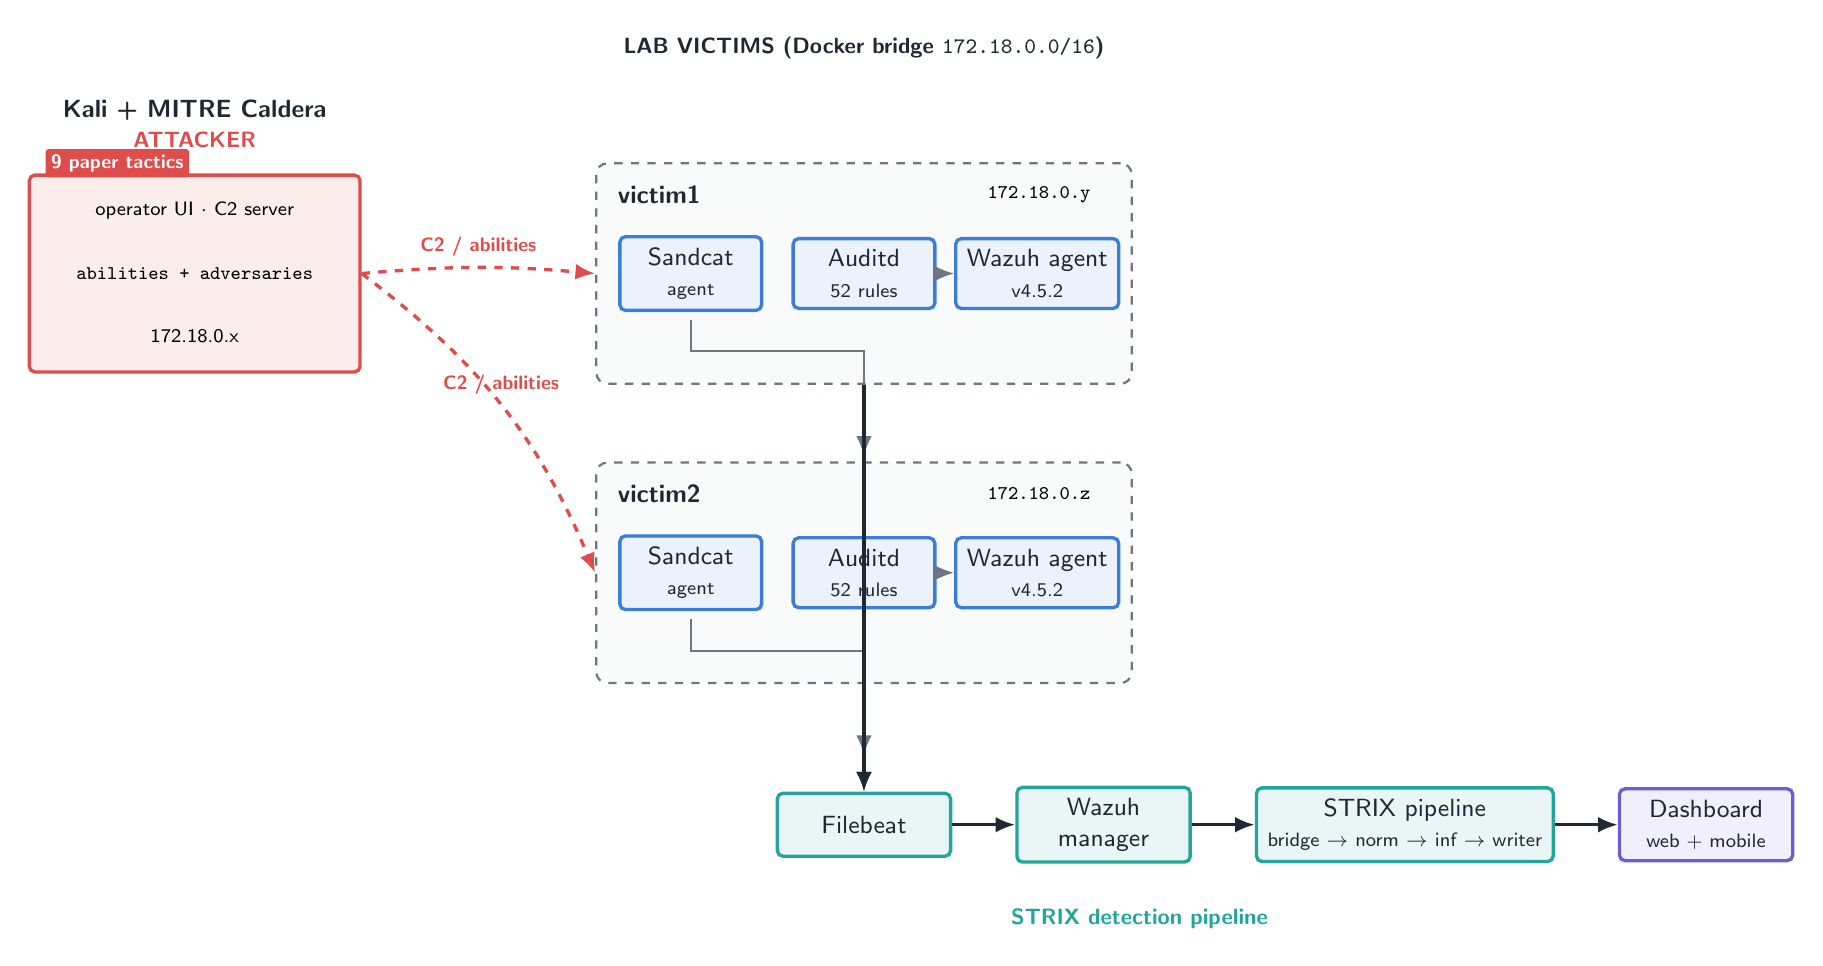
\begin{tikzpicture}[node distance=10mm]

% ─── Attacker side ───────────────────────────────────────────────
\node[ext, minimum width=42mm, minimum height=25mm] (caldera) {};
\node[title,font=\sffamily\bfseries\small] at ([yshift=8mm]caldera.north) {Kali + MITRE Caldera};
\node[font=\sffamily\scriptsize] at ([yshift=8mm]caldera.center) {operator UI \(\cdot\) C2 server};
\node[font=\sffamily\scriptsize\ttfamily] at ([yshift=0mm]caldera.center) {abilities + adversaries};
\node[font=\sffamily\scriptsize] at ([yshift=-8mm]caldera.center) {172.18.0.x};

% Tactic chips inside Caldera
\node[badge=strixRed, anchor=west] at ([xshift=-19mm,yshift=14mm]caldera.center) {9 paper tactics};

% ─── Two victim hosts ────────────────────────────────────────────
\foreach \i/\name/\ip/\yc in {1/victim1/172.18.0.y/0, 2/victim2/172.18.0.z/-3.8} {
  \node[group, minimum width=68mm, minimum height=28mm] (v\i) at (8.5,\yc) {};
  \node[title, font=\sffamily\bfseries\small] at ([yshift=10mm,xshift=-26mm]v\i.center) {\name};
  \node[font=\sffamily\scriptsize\ttfamily, anchor=east] at ([yshift=10mm,xshift=30mm]v\i.center) {\ip};
  \node[source, minimum width=18mm] (sand\i) at ([xshift=-22mm,yshift=0mm]v\i.center) {Sandcat\\\scriptsize agent};
  \node[source, minimum width=18mm] (aud\i) at ([xshift=0mm,yshift=0mm]v\i.center) {Auditd\\\scriptsize 52 rules};
  \node[source, minimum width=18mm] (wag\i) at ([xshift=22mm,yshift=0mm]v\i.center) {Wazuh agent\\\scriptsize v4.5.2};
  \draw[edge] (sand\i.south) ++(0,-1mm) -- ++(0,-4mm) -| ([yshift=-9mm]v\i.south) ;
  \draw[edge] (aud\i) -- (wag\i);
}

% ─── Telemetry pipeline (bottom) ─────────────────────────────────
\node[worker, minimum width=22mm] (fb) at (8.5,-7) {Filebeat};
\node[worker, minimum width=22mm, right=8mm of fb] (wm) {Wazuh\\manager};
\node[worker, minimum width=22mm, right=8mm of wm] (strix) {STRIX pipeline\\\scriptsize bridge $\to$ norm $\to$ inf $\to$ writer};
\node[ui, minimum width=22mm, right=8mm of strix] (dash) {Dashboard\\\scriptsize web + mobile};

\draw[edgeStrong] (v1.south) -- ++(0,-2mm) -| (fb.north);
\draw[edgeStrong] (v2.south) -- ++(0,-2mm) -| (fb.north);
\draw[edgeStrong] (fb) -- (wm);
\draw[edgeStrong] (wm) -- (strix);
\draw[edgeStrong] (strix) -- (dash);

% Caldera → victims attack arrows
\foreach \i in {1,2} {
  \draw[edgeStrong, draw=strixRed, dashed]
    (caldera.east) to[bend left=\i*10-5] node[midway, above, font=\sffamily\scriptsize\bfseries, text=strixRed]
    {C2 / abilities} (v\i.west);
}

% ─── Caption labels ──────────────────────────────────────────────
\node[font=\sffamily\bfseries\footnotesize, text=strixRed, anchor=south]
  at ([yshift=2mm]caldera.north) {ATTACKER};
\node[font=\sffamily\bfseries\footnotesize, text=strixDark, anchor=south]
  at (8.5, 2.6) {LAB VICTIMS (Docker bridge \texttt{172.18.0.0/16})};
\node[font=\sffamily\bfseries\footnotesize, text=strixGreen]
  at (12, -8.2) {STRIX detection pipeline};

\end{tikzpicture}
\end{document}
